%-----------------------------CAPITOLO 3
Come detto nella sezione~\ref{sec:BARIONE/MESONE}, $D^{0}$ e $\Lambda_{c}^{+}$ sono rispettivamente il mesone e il barione più leggeri contenenti un quark charm $c$ e per questo sono più abbondanti ad essere prodotti. Possono essere identificati nell'esperimento ALICE in un ampio intervallo di momento trasverso per cui si prestano molto bene per lo studio del loro rapporto di produzione.

L'identificazione avviene mediante la ricostruzione dei loro decadimenti carichi in volo. Le caratteristiche fisiche principali del $\Lambda_{c}^{+}$ sono un contenuto di quark $udc$, una massa di \qty{2286.46(0.14)}{\mega \eV \per \clight^2}, un $I\,(J^P) = 0\,({\frac{1}{2}}^{+})$ e una vita media di \qty{2.024(0.031)e-13}{\second}.

La $\Lambda_{c}^{+}$ possiede diversi \textit{canali di decadimento}, ma l'esperimento ALICE ne analizza tre, due adronici e uno semileptonico:
\begin{align}
    \Lambda_{c}^{+} & \to p K^{-} \pi^{+} 
    \label{eq:3-Lambda+c-decay-channel-pKpi} \\
    %
    \Lambda_{c}^{+} & \to p K^{0}_{S}
    \label{eq:3-Lambda+c-decay-channel-pK0S} \\
    %
    \Lambda_{c}^{+} & \to \Lambda e^{+} \bar{\nu}_{e}
    \label{eq:3-Lambda+c-decay-channel-Lambdae+nue}
\end{align}

I Branching Ratio (BR) di questi canali di decadimento, ovvero le \textit{probabilità} di decadimento di questi canali, sono rispettivamente:
\begin{itemize}
    \item[-] \qty{6.28(0.32)}{\percent} per il canale~\ref{eq:3-Lambda+c-decay-channel-pKpi},

    \item[-] \qty{1.59(0.08)}{\percent} per il canale~\ref{eq:3-Lambda+c-decay-channel-pK0S} e

    \item[-] \qty{3.60(0.40)}{\percent} per il canale~\ref{eq:3-Lambda+c-decay-channel-Lambdae+nue}.
\end{itemize}
Nella presente tesi viene preso in considerazione \textit{solamente} il canale di decadimento~\ref{eq:3-Lambda+c-decay-channel-pK0S} $\Lambda_{c}^{+} \to p K^{0}_{S}$ rappresentato in
figura~\ref{fig:3-1-Lambda+c-decay}.

Il punto in cui avviene la collisione ad alta energia tra due protoni dei fasci collidenti viene detto \textit{vertice primario}, nella figura~\ref{fig:3-1-Lambda+c-decay} rappresentato in rosso, con la conseguente formazione del barione $\Lambda_{c}^{+}$. In seguito la $\Lambda_{c}^{+}$ decade per \textit{interazione debole} nel punto detto vertice secondario, rappresentato in verde in figura, con le particelle figlie che sono rispettivamente un protone $p$ che è stabile e un mesone $K^{0}_{S}$ che a sua volta decade per interazione debole in due pioni carichi $\pi^{+} \pi^{-}$ con un BR del \qty{69.2(0.05)}{\percent}. Sono questi ultimi due che vengono effettivamente rilevati dal rivelatore microvertice di ALICE.

\begin{figure}[t]
    \centering
    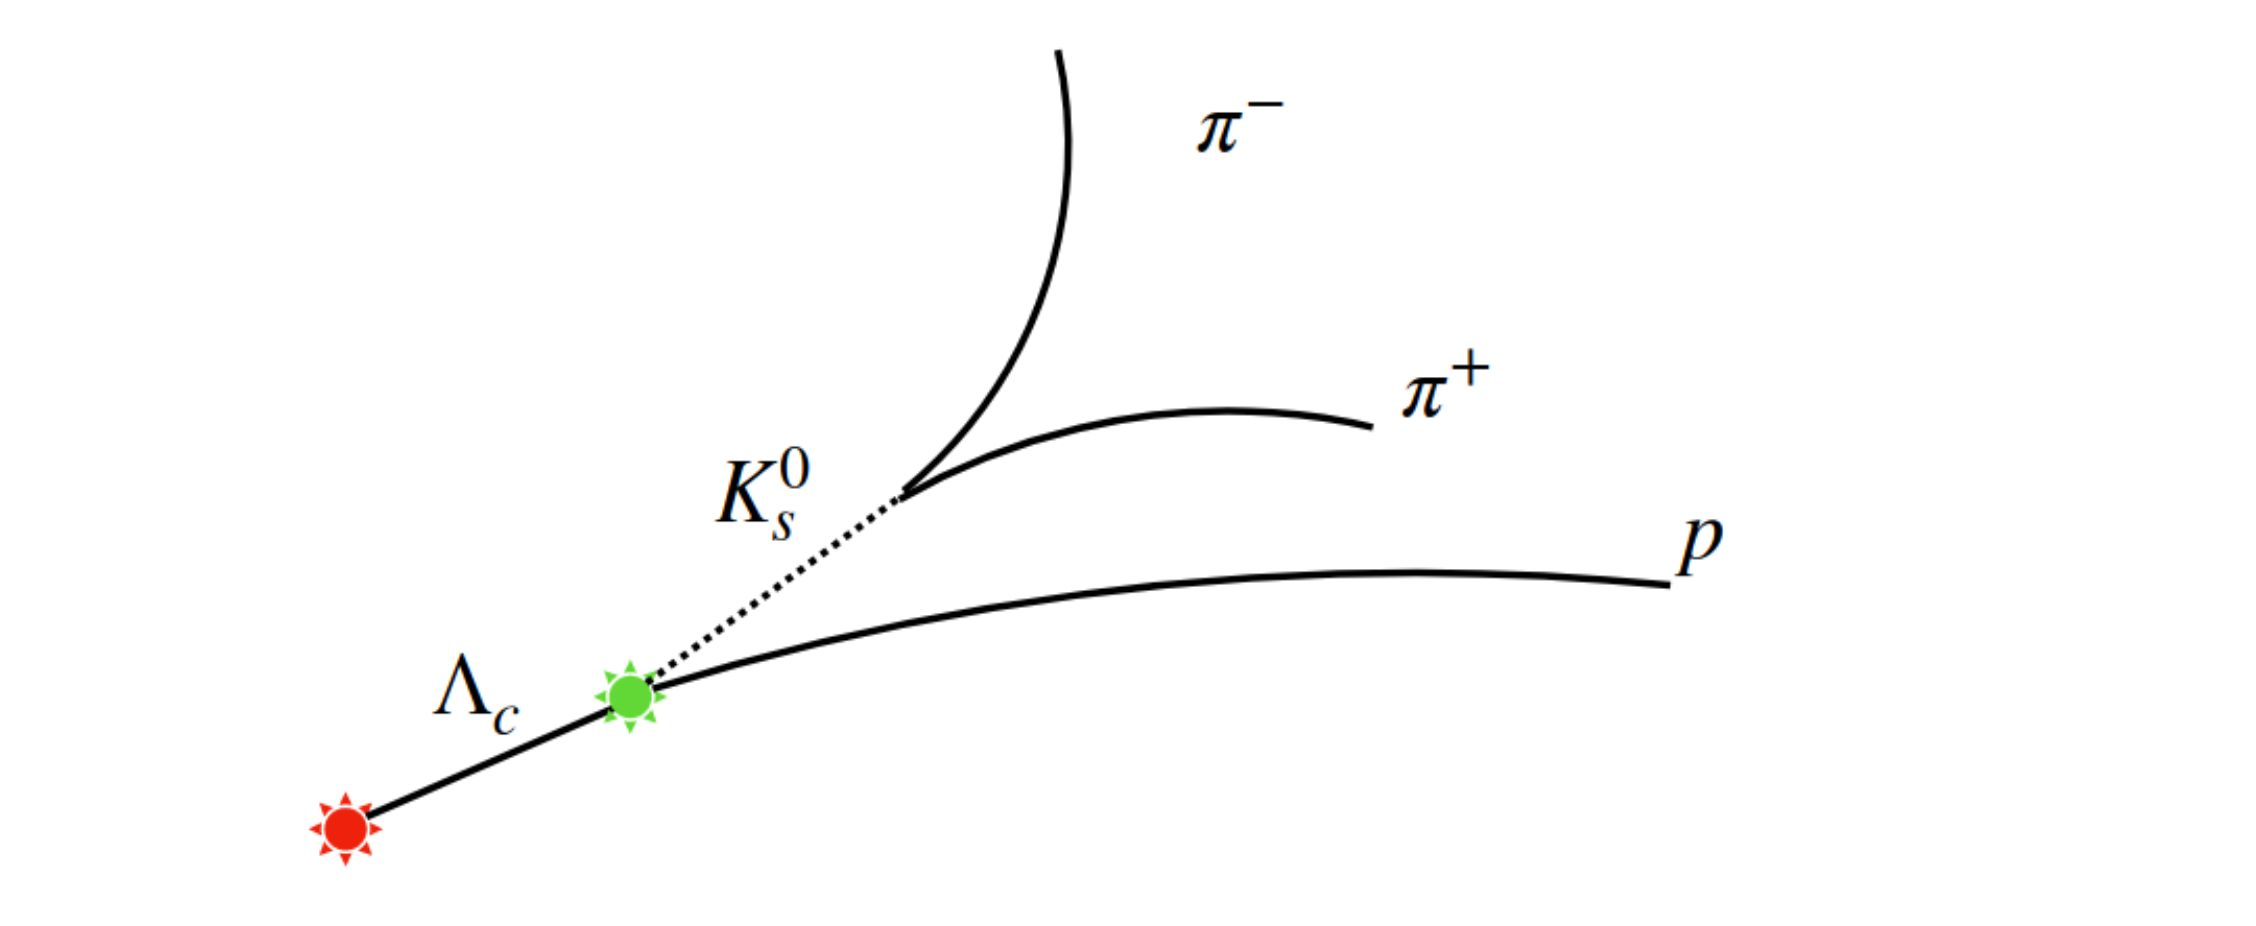
\includegraphics[width=1\linewidth]{res/fig/3-chapter/1-Lambda+c-decay.jpg}
    \caption{Rappresentazione grafica del decadimento del barione $\Lambda_{c}^{+}$ secondo il canale di decadimento~\ref{eq:3-Lambda+c-decay-channel-pK0S}, $\Lambda_{c}^{+} \to p K^{0}_{S}$~\cite{Fusconi_2022}.}
    \label{fig:3-1-Lambda+c-decay}
\end{figure}
% FALLO COL PACCHETTO DEI DIAGRAMMI DI FEYMAN

La principale sfida nell’analisi di questa particella è rappresentata dalla sua \textit{brevissima vita media}. Il barione $\Lambda_{c}^{+}$ ha un $c \tau =$ \qty{60}{\micro \meter} e quindi in media decade dopo aver percorso una distanza inferiore alla precisione dei rivelatori di microvertice di ALICE che si attesta intorno ai \qty{100}{\micro \meter} per impulsi trasversi $p_{T} \approx$ \qty{1}{\giga \eV \per \clight}. Questa situazione rende \textit{impossibile} la distinzione netta tra vertice primario e vertice secondario: tale complicazione rende l’analisi considerevolmente più complessa.

Dal momento che non è possibile discriminare tra particelle provenienti dal vertice primario e dal vertice secondario, è necessario implementare metodi più avanzati per separare le particelle effettivamente prodotte dal decadimento di una $\Lambda_{c}^{+}$ dal fondo (detto anche background). Questo fondo è costituito da tutte le possibili combinazioni di particelle che \textit{non} derivano dal decadimento di una $\Lambda_{c}^{+}$, ma che presentano caratteristiche simili a quelle che effettivamente lo sono e che, se combinate, forniscono un valore di massa invariante \textit{accidentalmente} simile a quello della massa di una $\Lambda_{c}^{+}$.

A tale scopo, risulta particolarmente utile l’utilizzo di tecniche basate sul Machine Learning. In questa tesi, è stata impiegata una rete neurale che fa utilizzo delle librerie Keras e TensorFlow di Python.

\newpage

\section{Dati e variabili fisiche degli eventi}
    Il campione di dati utilizzato per gli eventi di segnale è costituito da eventi simulati dal generatore Monte Carlo PYTHIA8~\cite{PYTHIA8_2013_data_simul}. In queste simulazioni, per aumentare la statistica, è stato posto il vincolo che ci sia \textit{almeno una} $\Lambda_{c}^{+}$ che decade secondo il canale di decadimento di nostro interesse tra tutte quelle che vengono generate. Per ottenere una simulazione ancora più fedele sono stati ``inseriti'' i comportamenti dei rivelatori che compongono l’esperimento ALICE in modo da simulare nel modo più verosimile possibile le interazioni delle particelle con i materiali di cui sono costituiti tali rivelatori, nonché la formazione dei loro segnali di risposta. La simulazione del rivelatore ALICE e la propagazione delle particelle è stata fatta utilizzando il software GEANT3~\cite{GEANT3_1994}.

    Il campione di dati utilizzato per il fondo, background, invece è stato ottenuto dalle misure stesse di ALICE, prese nella seconda fase di presa dati (RUN 2), avvenuta negli anni dal 2016 al 2018. Negli eventi dei dati reali, sono state però selezionate \textit{solo} candidate con una massa invariante ricostruita \textit{non} compatibile con la massa di una vera $\Lambda_{c}^{+}$.
    
    Come spiegato più ampiamente nelle sezioni successive, il Machine Learning~(ML) è lo studio di algoritmi capaci di imitare o trovare patterns nel campione di training attraverso l’esperienza. Un algoritmo di ML prende in input un insieme di variabili e applica delle funzioni per distinguerle nelle categorie conosciute. Si capisce dunque che la scelta di queste \textit{variabili di input} è di grande importanza e una \textit{buona} scelta permette all’algoritmo di separare le classi di eventi in segnale e fondo in maniera più efficiente.
    
    Prendendo come riferimento la figura~\ref{fig:3-1-Lambda+c-decay}, si parlerà di protone $p$ potenzialmente prodotto come di particella \textit{bachelor} e di $K^{0}_{S}$ potenzialmente prodotta come di particella~$V^{0}$. Le variabili fisiche degli eventi registrate dai diversi rivelatori e dell’esperimento ALICE che verranno utilizzate per allenare la rete neurale sono riportate nella seguente tabella~\ref{tab:3-1-vars}. Il nome che compare nella colonna ``Variabile fisica'' è quello utilizzato nel codice di analisi. La figura~\ref{fig:3-2-vars-histogram} mostra invece le distribuzioni di segnale e fondo di tutte le variabili in input per candidate $\Lambda_{c}^{+}$ ricostruite con un impulso trasverso nel range $1 < p_{T} < 2$ \unit{\giga \eV \per \clight}.

    \begin{table}[p]
        \centering
        \begin{tabular}{|>{\centering\arraybackslash}m{3cm}|>{\centering\arraybackslash}m{8.2cm}|>{\centering\arraybackslash}m{3cm}|}
            \hline
            \textbf{Variabile fisica} & \textbf{Descrizione} & \textbf{Valore} \\ 
            \hline
            \texttt{massK0S} & \textit{massa invariante} della particella $V^{0}$, ottenuta a partire dalle tracce ricostruite delle figlie & \qty{497}{\mega \eV \per \clight^2} \\ 
            \hline
            \texttt{tImpParBach} & \textit{parametro d'impatto} della particella bachelor definito come la distanza minima tra la traccia del bachelor e il vertice primario & \\ 
            \hline
            \texttt{tImpParV0} & \textit{parametro d'impatto} della particella $V^{0}$ & \\ 
            \hline
            \texttt{ctK0S} & $c \tau$ della particella $V^{0}$ assumendo che la sua massa sia quella di una $K^{0}_{S}$ & \qty{2.68}{\centi \meter} \\ 
            \hline
            \texttt{cosPAK0S} & \textit{coseno dell'angolo} tra la direzione della particella $V^{0}$ e la congiungente tra il vertice primario e il secondario & vicino all'unità \\ 
            \hline
            \texttt{nSigmapr} & \textit{probabilità}, in unità di deviazioni standard, che la particella bachelor sia effettivamente un protone ottenuta combinando le informazioni dei rivelatori TOF e TPC di ALICE (somma in quadratura delle due probabilità o solo probabilità fornita dalla TPC per candidate in cui l'informazione del TOF sia assente) & \\ 
            \hline
            \texttt{dcaV0} & Distance of Closest Approach, ovvero \textit{distanza minima} tra le tracce ricostruite delle due figlie della particella V$^{0}$ & \\ 
            \hline
        \end{tabular}
        \caption{Nomi, descrizioni e valori delle variabili fisiche utilizzate nell’allenamento della rete neurale.}
        \label{tab:3-1-vars}
    \end{table}
    
    \begin{figure}[p]
        \centering
        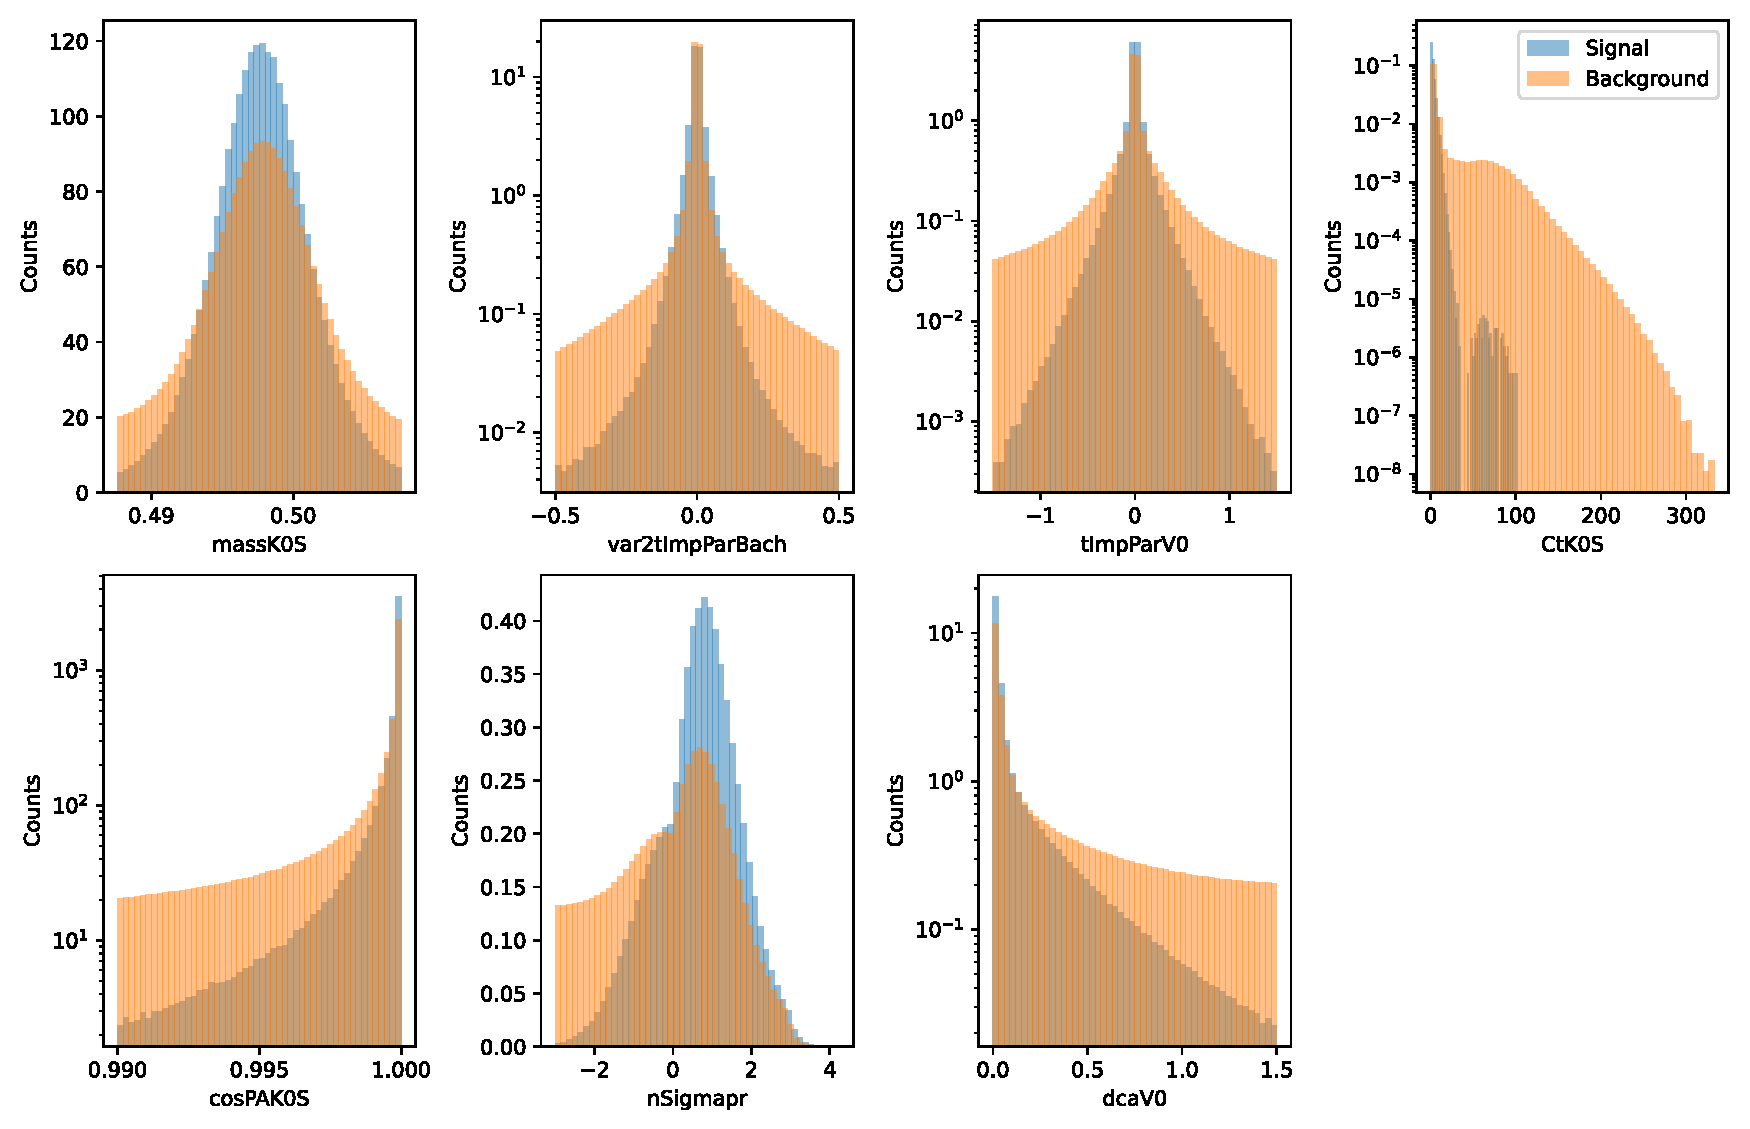
\includegraphics[width=1\linewidth]{res/fig/3-chapter/2-vars-histogram.pdf}
        \caption{Variabili utilizzate per il classificazione degli eventi, viene messa in luce la differenza tra il segnale e il background.}
        \label{fig:3-2-vars-histogram}
    \end{figure}

\clearpage

\section{Componenti software}
    Presentiamo brevemente le componenti software utilizzate per realizzare la rete neurale e per allenarla coi Data Trees forniti dall’esperimento ALICE.

    \subsection{TensorFlow}
        TensorFlow~\cite{TensorFlow} è una libreria open-source per il calcolo, ed è particolarmente nota per le sue applicazioni nelle intelligenze artificiali (AI). È stata sviluppata da ricercatori e ingegneri del Google Brain team ed è utilizzata per sviluppare, allenare e distribuire modelli di machine learning: offre moduli, strumenti e risorse per la gestione dei dati, l’ottimizzazione dei modelli, il monitoraggio delle prestazioni e molto altro.

        La libreria include diverse funzioni che rendono più agevole per gli sviluppatori creare e implementare modelli avanzati di apprendimento automatico, in particolare quelli basati su reti neurali. Le reti neurali (Neural Network, NN) sono una classe di modelli di apprendimento automatico ispirati alla struttura e al funzionamento del cervello umano, sono particolarmente efficaci per compiti complessi come il riconoscimento di immagini e la comprensione del linguaggio naturale.

        TensorFlow supporta vari linguaggi di programmazione, tra cui Python, ed è inoltre presente un’API (Application Programming Interface) molto utile chiamata Keras~\cite{Keras}. Un’API è un’interfaccia che permette a programmi software differenti di comunicare tra loro, fornisce inoltre un’interfaccia tra il software a basso livello e quello ad alto livello semplificando notevolmente la fase di scrittura del codice di programmazione da parte dell’utente. Oggi esistono svariate API per la creazione di intelligenze artificiali, ne sono esempio le API di OpenAI di ChatGPT oppure le API di TensorFlow, come Keras, utilizzata in questa tesi per allenare la rete neurale.

    \subsection{Keras}
        Inizialmente, Keras è stato sviluppato come un’interfaccia indipendente che poteva funzionare con diverse librerie di backend, tra cui TensorFlow, Theano e Microsoft Cognitive Toolkit. Tuttavia, con il rilascio di TensorFlow 2.0, Keras è stato ufficialmente incorporato in TensorFlow come \texttt{tf.keras}: questo ha reso Keras l’API maggiormente utilizzata per TensorFlow, ovvero un’interfaccia per costruire e addestrare modelli di deep learning (DL).

        Per utilizzare Keras o più in generale il deep learning, in contesti dove si utilizza il framework ROOT scritto in C++ come in fisica delle particelle, è utile sapere analizzare e interpretare poche righe di codice per rendere agevoli delle analisi di strutture complesse di dati. In tali casi, si può sfruttare Keras per costruire modelli di reti neurali che aiutano nell’analisi multivariata dei dati e nella classificazione degli eventi come è stato fatto in questa tesi. Il codice di questa tesi è disponibile nella repository GitHub \href{https://github.com/giopedro92/bachelor-thesis-code}{\texttt{bachelor-thesis-code}}.

\section{Analisi preliminari: matrice di correlazione}
    Prima di eseguire il training vero e proprio, è stato necessario produrre le matrici di correlazione lineare delle variabili in input, sia per il segnale, sia per il fondo, figura~\ref{fig:3-4-correlation-matrix}. Lo studio di queste matrici è importante perché variabili altamente correlate potrebbero compromettere l'apprendimento della rete o aumentare di molto il tempo di allenamento che dipende tra le altre cose dal numero di variabili in input. In questo caso specifico le variabili non presentano eccessive correlazioni tra di loro.

    \begin{figure}[h!]
        \centering
        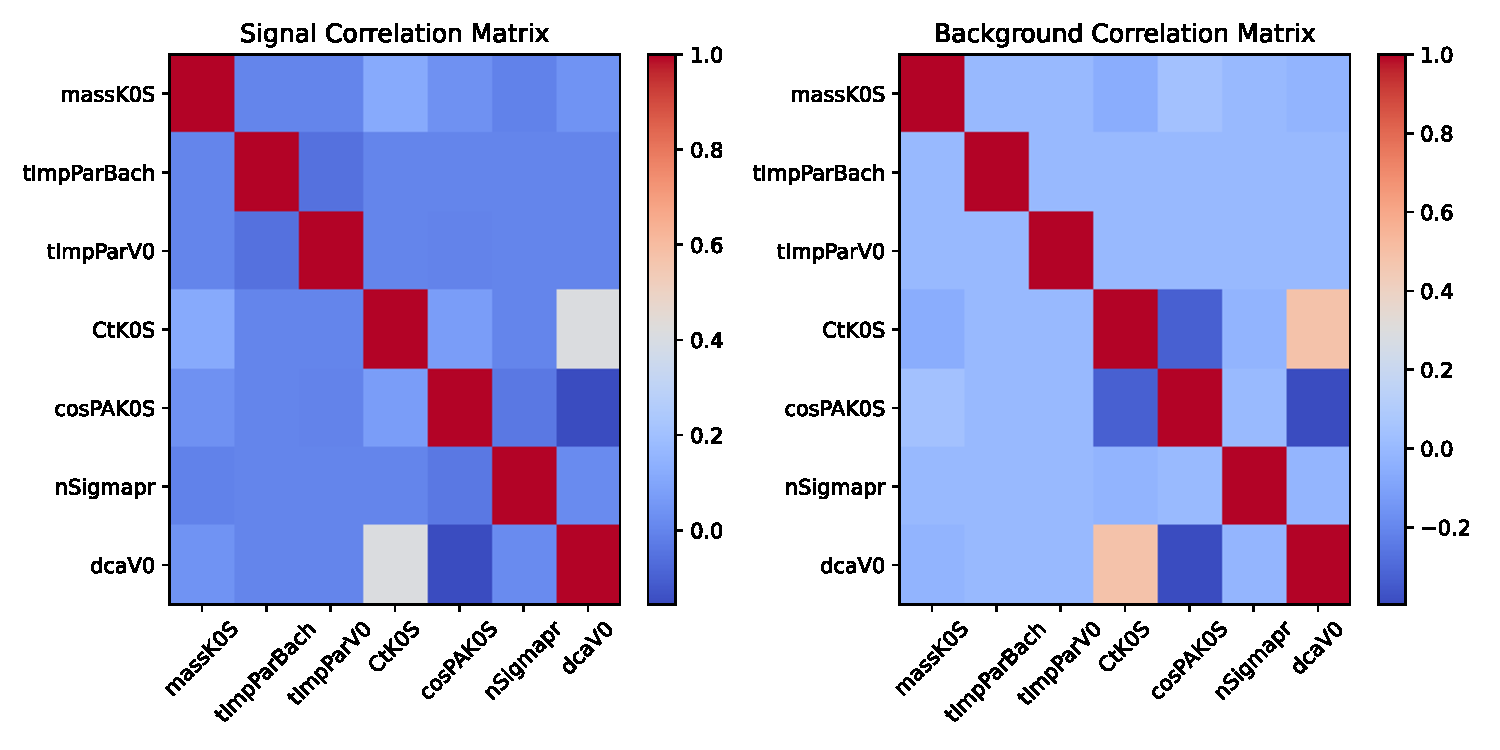
\includegraphics[width=1\linewidth]{res/fig/3-chapter/4-correlation-matrix.pdf}
        \caption{Matrici di correlazione lineare delle variabili in input a sinistra per il segnale e a destra per il fondo.}
        \label{fig:3-4-correlation-matrix}
    \end{figure}

\newpage

\begin{comment}
\section{Introduzione alla classificazione e applicazione delle reti neurali}
    È necessario realizzare la classificazione dei modelli da utilizzare per l’analisi multivariata. Ne elenchiamo i principali punti chiave: come primo passo bisogna estrarre, o meglio dire leggere, i dati sperimentali salvati nel ROOT file (dati acquisiti per gli eventi $pp$ dal rivelatore ALICE) e la simulazione da presentare come esempio alla rete neurale (questa simulazione è stata realizzata dalla collaborazione ALICE attraverso un generatore Monte Carlo PYTHIA 8 [26]);
    
    questi file sono organizzati in trees, che sono specifiche strutture di ROOT [27], dove in ogni ramo sono raccolte informazioni su variabili fisiche dei vari eventi.
    
    Il punto successivo è quello di organizzare e configurare queste variabili sul Data- Loader di TMVA al quale poi vengono forniti i file di input (nel nostro caso dataNew.root e signalNew.root). Di conseguenza si possono dunque preparare i trees di training e di test utilizzando il metodo specifico; in tutti questi casi di tiene conto solamente di eventi con impulso trasverso del segnale candidato ricostruito, pT , compreso tra 0 e 1 GeV /c.
    
    Prima di compilare si definisce il modello della rete neurale per poi salvarlo su un apposito file utilizzando specifiche funzioni di Keras. Infine si usa la funzione BookMethod di TMVA per imporre il tipo di classifier da utilizzare opportunamente configurato. Per comprendere meglio quest’ultimo punto si faccia riferimento al paragrafo 4.4.

    Utilizzando i files della classificazione si ottengono le varie matrici di correlazione e i grafici con le efficienze dei tagli da adoperare con un valore specifico stampato su terminale che rappresenta il taglio ottimale per eliminare più fondo possibile senza perdere troppo segnale.

    Il passo seguente è quello di applicare questo taglio a tutti gli eventi contenuti nel file con l’intero dataset da analizzare (dataNew.root) eseguendo un loop che confronta tutti i dati e li elimina nel caso non soddisfino i requisiti del taglio. Per fare questo si estrae il tree da prendere in considerazione dal file dataNew.root e lo si salva attribuendo corretamente i nome delle variabili attraverso un loop che scorre i rami del tree. Utilizzando la funzione BookMVA per definire i pesi che si sono calcolati nel punto precedente, si possono infine creare gli istogrammi riempiti solamente con le masse invarianti che soddisfano i requisiti di taglio. si possono effettuare dei fit alla distribuzione di massa invariante per calcolare il numero di $\Lambda_{c}^{+}$ prodotte in tali collisioni.

    \begin{figure}[h]
        \centering
        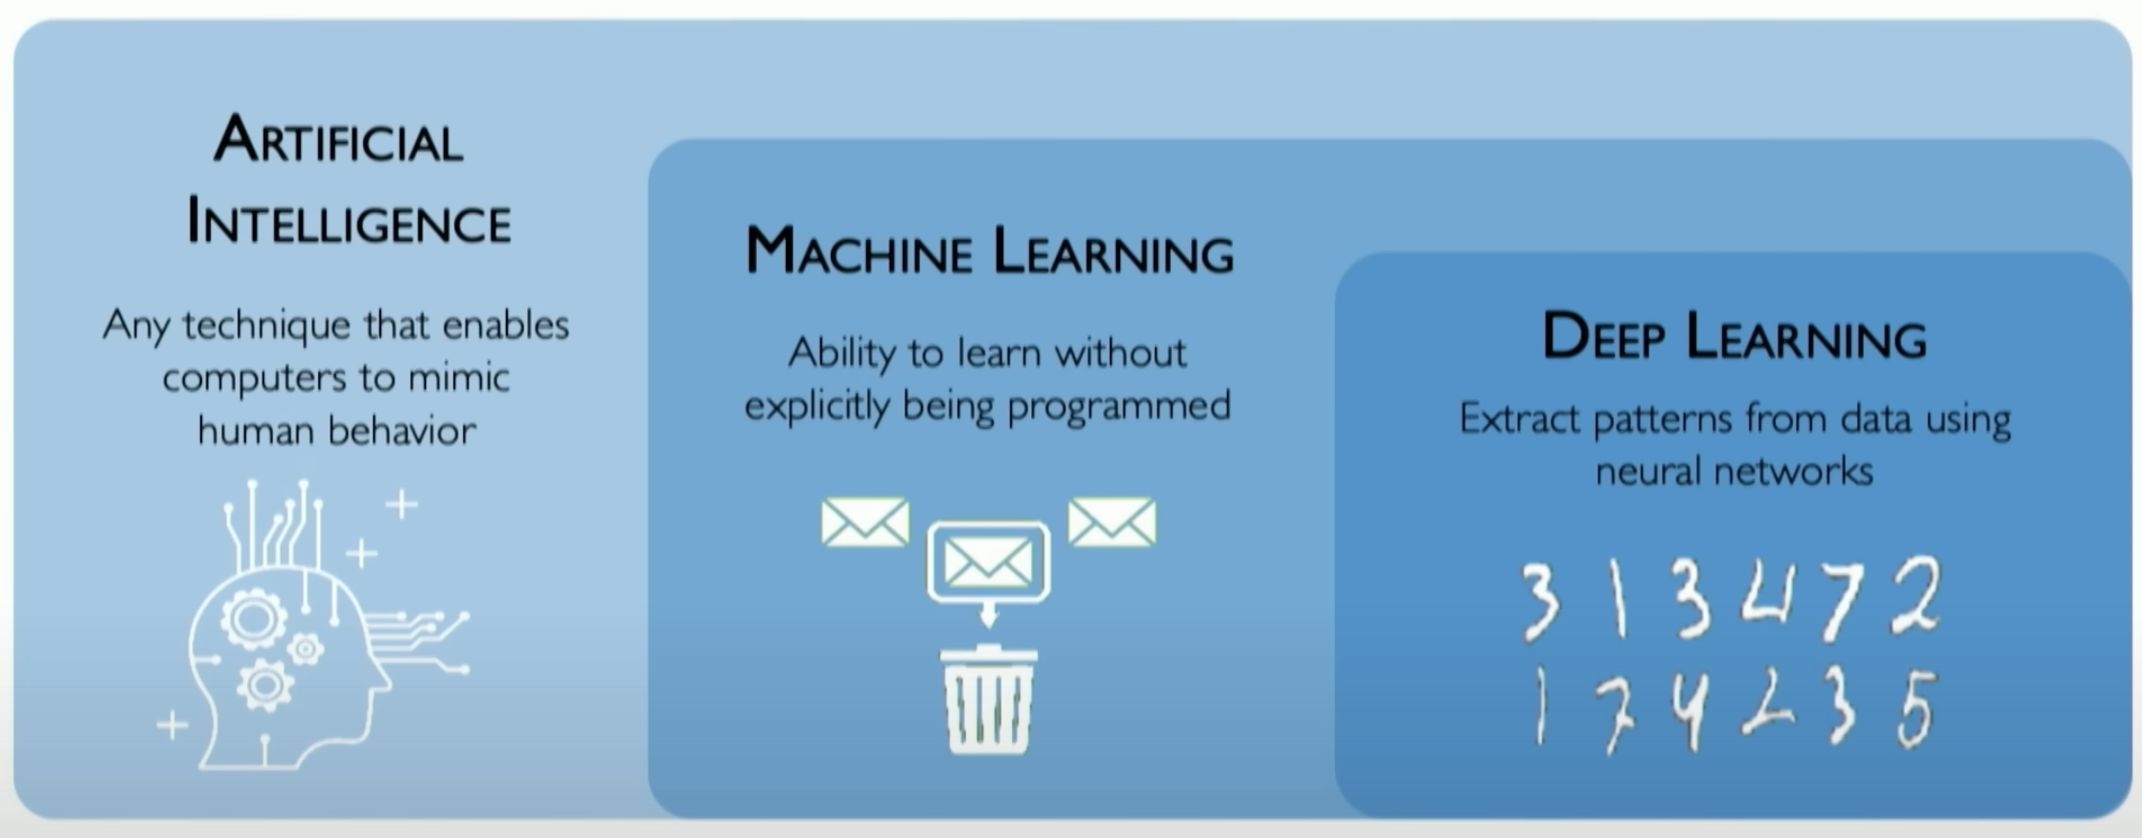
\includegraphics[width=0.5\linewidth]{res/fig/3-chapter/3-ai-ml-dl.jpg}
        \caption{Classificazione del DL nelle AI come spiegato nella lezione del MIT~\cite{ASWTKGAR_2020_MIT_AI_ML_DL}.}
        \label{fig:3-3-ai-ml-dl}
    \end{figure}
\end{comment}

\newpage

\section{Il modello di Neural Network (NN)}
    Il codice è stato distribuito in 4 file, il \texttt{main.py} e
    \begin{description}
        \item[\texttt{DataPreparation.py}] contenente la classe \texttt{DataPreparation} con al suo interno le funzioni \texttt{load\_data} per caricare i dati dai tree e \texttt{prepare\_data} per normalizzarli,

        \item[\texttt{Classifier.py}] contenente le classi
        \begin{description}
            \item[\texttt{SignalBackgroundClassifier}] con al suo interno le funzioni \texttt{train\_classifier} per allenare la rete e \texttt{evaluate\_classifier} per valutare l'allenamento,

            \item[\texttt{NeuralNetwork}] con al suo interno le funzioni \texttt{build\_model} e \texttt{train\_classifier} per la costruzione e l'allenamento del modello di rete neurale e

            \item[\texttt{Additional\_evaluation}] con la funzione \texttt{plot\_feature\_importance} per stampare l'importanza delle variabili del training,
        \end{description}
        
        \item[\texttt{MetricPrinter.py}] contenente la classe \texttt{PrintMetrics} per stampare le metriche dell'allenamento con al suo interno le funzioni \texttt{plot\_roc\_curve} e \texttt{print\_metrics}.
    \end{description}
    
    Il modello di rete neurale è il cosiddetto \texttt{Sequential}, che ha il vantaggio di essere semplice da costruire per chi è alle prime armi con la costruzione di reti neurali. Presenta inoltre una struttura lineare dove ogni strato ha un input e un output e l’output di uno strato diventa l’input dello strato successivo. Un’altra caratteristica importante è che questo modello è utilizzato prevalentemente per costruire reti neurali feedforward, ovvero dove i dati si muovono in una direzione, dall’input all’output, senza cicli~\cite{Manaswi_2018}.

\begin{comment}
% inserici cose tradotte
In questo caso il modello realizzato ha 

    In questo caso il modello realizzato è a due strati densi, ossia completamente connessi: il primo strato è a 64 neuroni con funzione di attivazione ReLU e le 7 variabili d’ingresso, il secondo strato ha 1 neuroni, uno per ciascuna classe di output, con funzione di attivazione Sigmoide .

\textbf{NOTA A PIÈ DI PAGINE SULLA RELU}

    La ReLU è una funzione di attivazione fondamentale nel campo del deep learning, che offre un buon compromesso tra non-linearità, efficienza computazionale e capacità di apprendimento. Una funzione di attivazione in una rete neurale è una componente cruciale che decide se un neurone deve essere attivato o meno, è ciò che consente alle reti neurali di catturare relazioni complesse e non lineari nei dati. [29]

\end{comment}

    Di seguito sono presenti le righe di codice per la costruzione del modello:
    \begin{lstlisting}[language=Python, style=myPython]
def build_model(self,
                X_train,
                neurons,
                drop_out,
                learning_rate):    
    
    model = keras.Sequential([
                layers.Input(
                    shape = (X_train.shape[1])),
                # layer di input, shape = dimensione dei dati
                layers.Dense(
                    neurons,
                    activation = "relu"),
                # layer collegati a tutti i neuroni
                layers.Dropout(
                    drop_out),
                # spegne un certo numero di neuroni
                # per non influenzare troppo la rete
                layers.Dense(
                    neurons,
                    activation = "relu"),
                layers.Dropout(
                    drop_out),
                layers.Dense(
                    1,
                    activation = "sigmoid")])

    optimizer = keras.optimizers.Adam(
                    learning_rate = learning_rate)
                # usa optimizer Adam

    model.compile(
        optimizer = optimizer,
        loss      = "binary_crossentropy",
        metrics   = ["accuracy"])
        # loss function adeguata per il problema
return model
    \end{lstlisting}
    
    L’addestramento di una rete neurale è un processo complesso che coinvolge l’uso di algoritmi di ottimizzazione per regolare i pesi della rete in modo che possa eseguire correttamente un determinato compito. In generale l’obbiettivo è quello di minimizzare un gradiente rispetto a tutti i parametri del modello.

    Il \textit{Stocastic Gradient Descent} (SGD) è una variante dell’algoritmo di discesa del gradiente utilizzato per l’ottimizzazione delle reti neurali e in altri modelli di apprendimento automatico. Questo è caratterizzato da un processo randomico dell’analisi del gradiente e dal fatto che non analizza l’intero set di dati per aggiornare i pesi dei parametri ma appunto esegue l’analisi su dei batch che sono sottinsiemi randomici. Per ogni \textit{batch}, la rete neurale esegue una previsione e in seguito ne calcola la perdita ovvero la differenza tra la previsione e il valore vero, di conseguenza calcola il gradiente della funzione di perdita rispetto ai pesi. Infine, aggiorna i pesi in direzione opposta alla crescita del gradiente per ridurre la perdita. Idealmente l’addestramento continua fino a quando la rete non mostra più miglioramenti significativi sul set di validazione, indicando che ha raggiunto una buona generalizzazione.

    La \textit{crossentropy} è una misura della differenza tra due distribuzioni di probabilità: la distribuzione reale dei dati e la distribuzione prevista dal modello. Nella classificazione, la crossentropy è comunemente usata come funzione di perdita: misura quanto efficacemente il modello preveda i dati sperimentali e ne penalizza le previsioni che sono lontane dalla verità effettiva. In librerie come TensorFlow e Keras, la crossentropy è implementata come una funzione di perdita predefinita e ne si può specificare il tipo durante la compilazione del modello come si può vedere nelle righe di codice. Esistono due forme principali di crossentropy utilizzate: quella qui utilizzata è detta \textit{binaria} utilizzata per problemi in cui la risposta può appartenere solamente a due classi possibili, ad esempio vero o falso, mentre un'altra possibile è detta categorical crossentropy la quale è utilizzata per problemi di classificazione multivariata.

\newpage

\section{Scelta dei Classifiers per il modello}
    Per effettuare il training delle varie reti neurali sono stati utilizzati diversi classifiers, ovvero metodi di configurazione e addestramento del modello, ognuno dei quali con caratteristiche differenti.

    Un \textit{batch} è un sottoinsieme di esempio per l’addestramento utilizzato in un’unica iterazione dell’algoritmo di apprendimento; la dimensione di questo determina l’efficacia con cui si minimizza il gradiente stocastico: batches di dimensione ridotta possono portare a una stima più rumorosa del gradiente ma possono anche aiutare la rete a generalizzare meglio l’evento e a uscire dai minimi locali durante l’addestramento. D’altra parte, batches più grandi forniscono una stima più accurata del gradiente ma possono essere computazionalmente più costosi e potrebbero portare a una convergenza in un minimo locale meno ottimale.

    Un’\textit{epoca} è un termine che si riferisce al completamento di un intero ciclo di passaggio attraverso un batch di dati di addestramento. Durante un’epoca l’algoritmo lavora attraverso ogni esempio di addestramento aggiornando i pesi della rete in base alla perdita calcolata per quegli esempi.

        \begin{table}[h]
            \centering
            \begin{tabular}{|>{\centering\arraybackslash}m{4.1cm}|>{\centering\arraybackslash}m{6cm}|>{\centering\arraybackslash}m{3.5cm}|}
                \hline
                \textbf{Parametro} & \textbf{Descrizione} & \textbf{Valore} \\
                \hline
                \texttt{epochs} & Numero di \textit{epoche} di addestramento per il modello & 10 \\
                \hline
                \texttt{batch\_size} & Dimensione del \textit{batch} durante l'addestramento & 32 \\
                \hline
            \end{tabular}
            \caption{Descrizione dei parametri del modello.}
        \end{table}

    Dopo diversi tentativi è stato individuato il valore di 10 epoche come il migliore per i dati su cui desideriamo allenare la rete.

\begin{comment}
\section{Training del modello}
    

    \subsection{Metriche attraverso le epoche}
        \textbf{ANCORA DA FARE IMMAGINE CON CODICE}
        
        \begin{figure}[h]
            \centering
            \includegraphics[width=0.5\linewidth]{res/fig/3-chapter/5-metrics-epochs.pdf}
            \caption{Caption.}
            \label{fig:enter-label}
        \end{figure}
\end{comment}

\newpage

\section{Verifica della correttezza del training}
    Durante l'allenamento la rete passa attraverso i dati di segnale e fondo che sono stati etichettati come 1 per il segnale e 0 per il fondo. La rete fa delle previsioni (assegnando valori 1 a quelli che pensa siano dati di segnale e 0 a quelli che pensa siano dati di fondo) che vengono poi validate da una parte dei dati su cui la rete non si allena.
    
    Esistono molti modi per valutare la bontà dell'allenamento della rete.

    \subsection{Confusion matrix (CM)}
        Indicando il segnale come 1 (positive) e il fondo come 0 (negative) e indicando con 1 (true) l'ipotesi di correttezza che la rete fa e 0 (false) l'errore rispetto alla previsione della rete, possiamo disporre su una matrice il numero di dati correttamente riconosciuti o meno, come mostrato in figura~\ref{fig:confusion-matrix}. Chiamiamo (i valori tra parentesi identificano l'elemento di matrice):
        \begin{description}
            \item[True Positive \,\,\,(TP \,1,1)] i dati di segnale correttamente riconosciuti,

            \item[True Negative \,(TN 0,0)] i dati di fondo correttamente riconosciuti,

            \item[False Positive \,\,\,(FP \,0,1)] i dati di fondo erroneamente classificati come segnale,

            \item[False Negative (FN \,1,0)] i dati di segnale erroneamente classificati come fondo.
        \end{description}
         
        \begin{figure}[h]
            \centering
            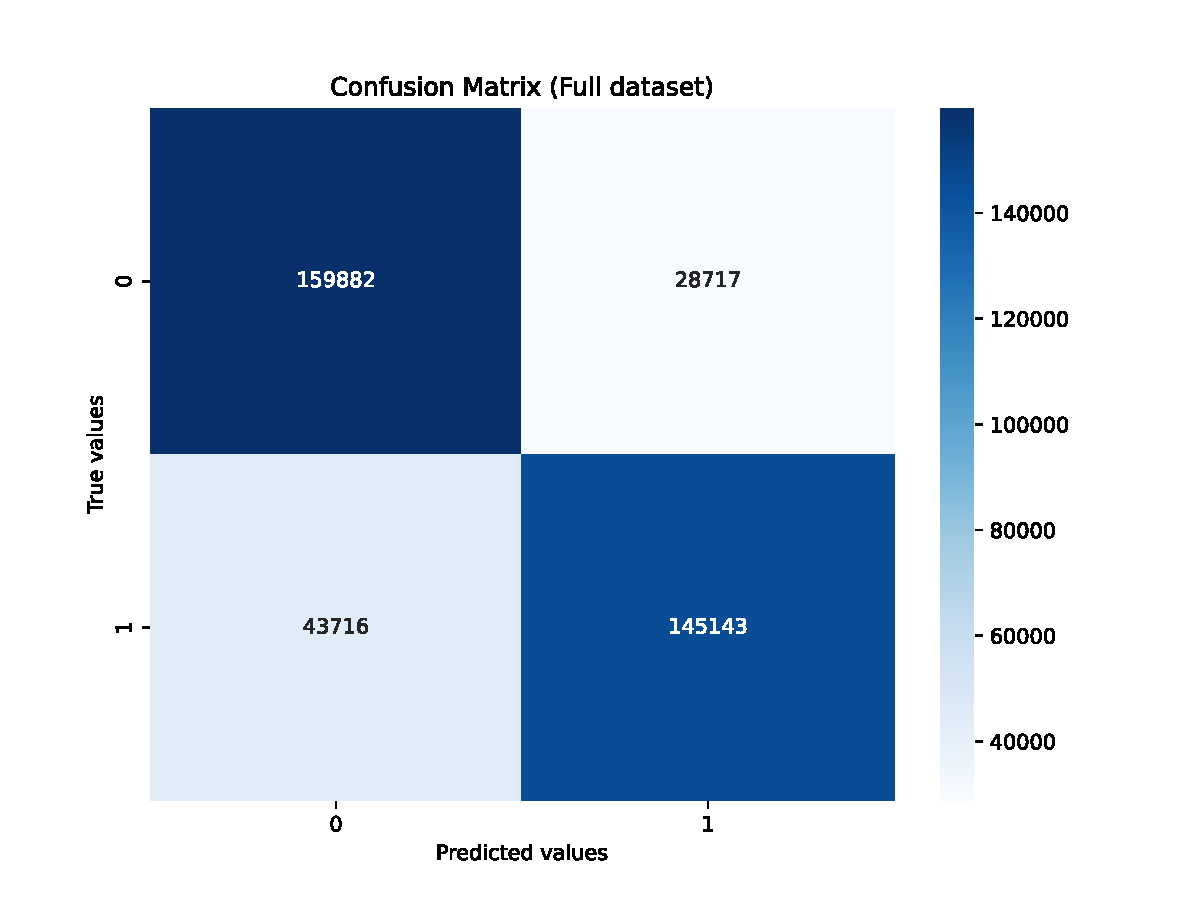
\includegraphics[width=0.80\linewidth]{res/fig/3-chapter/6-confusion-matrix.pdf}
            \caption{Confusion matrix dall'allenamento.}
            \label{fig:confusion-matrix}
        \end{figure}

\newpage

\section{Metriche}
    Utilizzando le variabili introdotte nella precedente sezione è possibile introdurre diverse metriche che forniscono maggiori informazioni legate alla matrice di correlazione tutte definite in \qtyrange[range-phrase = {,}, range-units = single, per-mode = symbol, range-units = bracket, range-open-bracket = [, range-close-bracket = ]]{0}{1}{}:
    \begin{description}
        \item[Precision] è definita come
        \begin{equation}
            \text{Precision} = \frac{\text{correttamente classificati come positivi}}{\text{tutti quelli classificati come positivi}} = \frac{TP}{TP + FP}
        \end{equation}
        ed è una misura della proporzione di esempi positivi classificati correttamente rispetto a tutti gli esempi classificati come positivi. In altre parole, ``Quanto è affidabile il modello quando prevede una classe positiva?''.

        \item[Accuracy] è definita come
        \begin{equation}
            \text{Accuracy} = \frac{\text{correttamente classificati}}{\text{tutti quelli classificati}} = \frac{TP + TN}{TP + TN + FP + FN}
        \end{equation}
        ed è una misura della proporzione di istanze correttamente predette (sia veri positivi che veri negativi) rispetto al numero totale di istanze.

        \item[Recall] (o tasso di veri positivi) è definita come
        \begin{equation}
            \text{Recall} = \frac{\text{correttamente classificati come positivi}}{\text{tutti i positivi}} = \frac{TP}{TP + FN}
        \end{equation}
        e misura la proporzione di esempi positivi classificati correttamente rispetto a tutti gli esempi positivi reali. In altre parole: ``Quanto è completo il modello nel trovare tutti gli esempi positivi?''.

        \item[Tasso di errore] definito come
        \begin{equation}
            \text{Err} = \frac{FP + FN}{TP + TN + FP + FN}
        \end{equation}
        e misura la percentuale di errore delle previsione sul numero totale delle istanze.

        \item[F1-score] è definita come
        \begin{equation}
            \text{F1} = 2 \cdot \frac{\text{precision} \cdot \text{recall}}{\text{precision} + \text{recall}} = \frac{TP}{TP + \frac{1}{2}\,(FP + FN)}
        \end{equation}
        ed è una sorta di ``media armonica'' tra la precisione e la recall. Fornisce una misura bilanciata di entrambe queste metriche risultando particolarmente utile quando si ha a che fare con dataset sbilanciati (cioè quando le classi non sono rappresentate in modo equo). Un buon F1-score indica che il modello ha sia un'alta precisione che un alto recall.
    \end{description}

    Un modello perfetto avrebbe zero falsi positivi e zero falsi negativi e pertanto avrebbe precisione, accuracy, recall e F1-score pari a 1, mentre il tasso di errore sarebbe pari a 0.
    
    Il modello ottenuto dalla rete neurale sviluppata ha restituito i seguenti valori per le metriche sopra enunciate (solo quelle implementate): $\text{accuracy}  =$ \num{0.808}, $\text{precision} =$ \num{0.835} e $\text{f1 score}  =$ \num{0.800}. I valori sono accettabili e comunque vicini all'unità.

\begin{comment}
    \begin{table}[h!]
        \centering
        \begin{tabular}{cc|cc|}
            \cline{3-4}
              &   & \multicolumn{2}{c|}{\textbf{Predicted labels}} \\ %\cline{3-4} 
              &   & \multicolumn{1}{c|}{\small{0}}       & \small{1}  \\ \hline
            \multicolumn{1}{|c}{\multirow{2}{*}{\textbf{True labels}}} & \small{0} & \multicolumn{1}{c|}{TN: 9113} & FP: 056 \\ 
            \cline{2-4} 
            \multicolumn{1}{|c}{} & {\small{1}} & \multicolumn{1}{c|}{FN: 0192} & TP: 716\\ 
            \hline
        \end{tabular}
        \caption{Confusion matrix obtained from this model.}
        \label{tab:conf-matrix}
    \end{table}
\end{comment}

\newpage

    \subsection{Ranking delle variabili}
        La rete può apprendere più informazioni per l'allenamento da una variabile piuttosto che da un'altra, per questo è utile produrre una grafico di ranking delle diverse variabili utilizzate per l'allenamento.
        
        In figura~\ref{fig:3-7-feature-importance} è riportato il ranking delle variabili di training del modello utilizzato. Non è stata compresa l'importanza tanto più grande della variabile \texttt{CtK0S} rispetto alle altre per l'addestramento: sembra essere stata ritenuta dalla rete molto più significativa nella distinzione del segnale dal fondo.
        
        \begin{figure}[h]
            \centering
            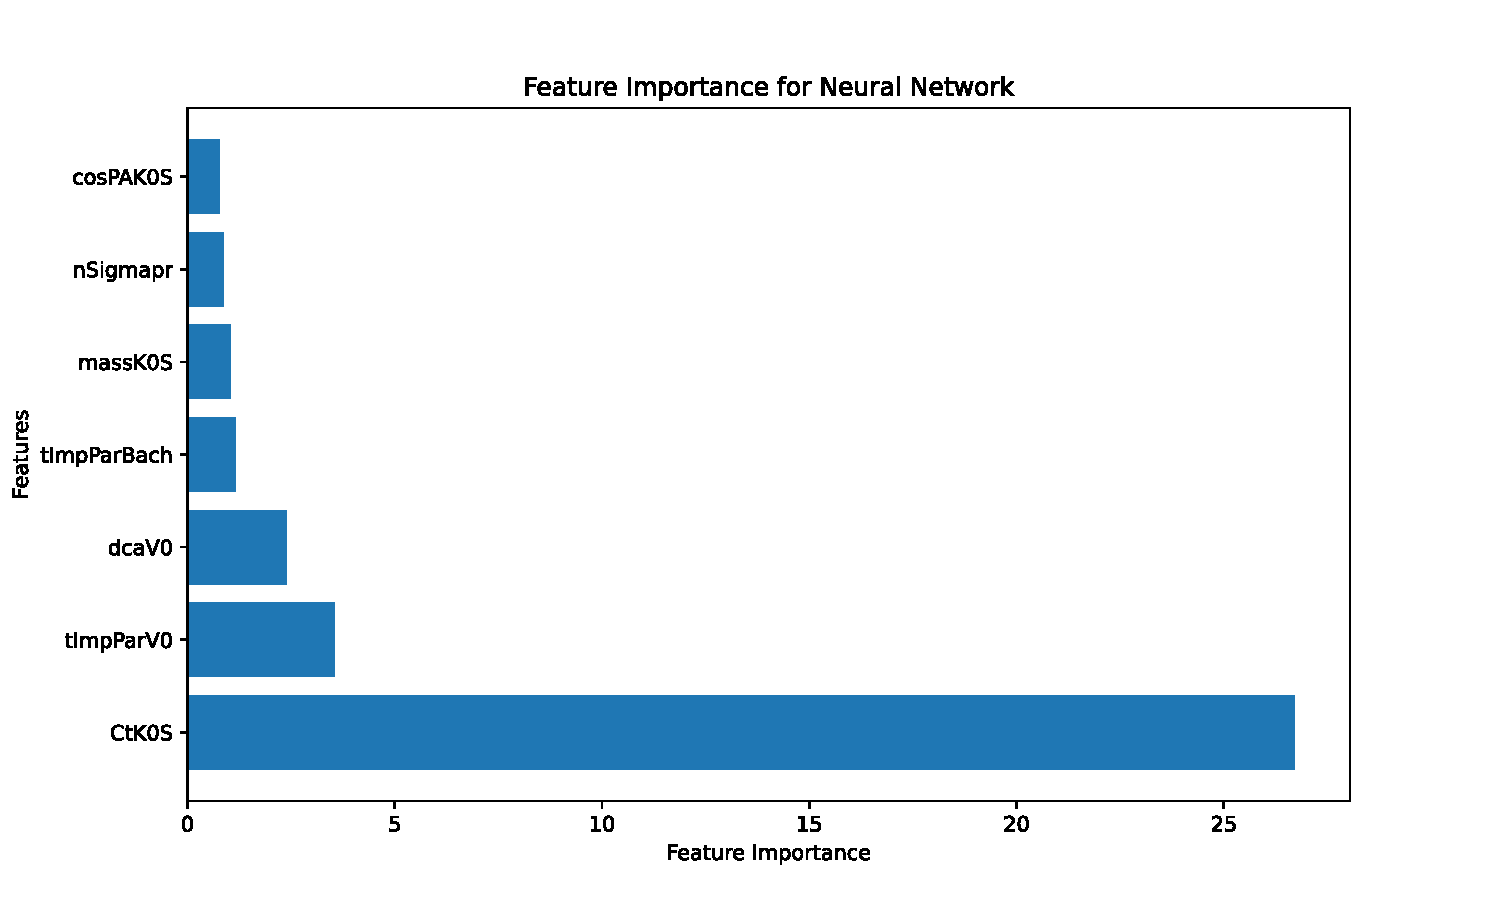
\includegraphics[width=1\linewidth]{res/fig/3-chapter/7-feature-importance.pdf}
            \caption{Ranking delle variabili di training.}
            \label{fig:3-7-feature-importance}
        \end{figure}

\newpage

    \subsection{Curva di ROC}
        La curva \textit{ROC} (Receiver Operating Characteristic) è uno strumento grafico utilizzato per valutare le prestazioni di un modello di classificazione binaria come il nostro. Viene tracciata confrontando la Sensibilità (o Recall) con la Specificità (o il complemento della Specificità, noto anche come Tasso di Falsi Positivi).

        Dopo l'allenamento la rete ha restituito la curva mostrata in figura~\ref{fig:ROC-curve}. Sull'asse orizzontale è rappresentato il True Positive Rate (TPR) definito come
        \begin{equation}
            \text{TPR} = \frac{\text{Veri Positivi}\ (TP)}{\text{Veri Positivi}\ (TP) + \text{Falsi Negativi}\ (FN)},
        \end{equation}
        mentre sull'asse delle ordinate è rappresentata la Background Rejection definita come il complemento del False Positive Rate (FPR):
        \begin{equation}
            \text{Background Rejection} = 1 - \text{FPR} = \frac{\text{Veri Negativi}\ (TN)}{\text{Veri Negativi}\ (TN) + \text{Falsi Positivi}\ (FP)}
        \end{equation}
        Questa misura rappresenta la proporzione di eventi negativi (background) correttamente identificati come tali dal modello.

        Questa rappresentazione può essere utile in applicazioni come la fisica delle particelle, dove il background rappresenta rumore o eventi non interessanti, e si desidera ridurre al minimo l'inclusione di questi eventi massimizzando l'identificazione di eventi significativi (segnale).

        Una curva vicina all'angolo superiore destro come quella ottenuta, indica un modello con ottime prestazioni, con alto TPR e alta Background Rejection (basso FPR).

        Attraverso l'analisi delle curve ROC si può valutare la capacità della rete neurale di classificare correttamente gli eventi calcolando l'\textit{area sottesa dalla curva ROC} (Area Under Curve, AUC). Il valore di AUC, compreso tra 0 e 1, equivale infatti alla \textit{probabilità} che il modello, se vengono forniti un esempio positivo e negativo scelto in modo casuale, assegni un \textit{valore del classificatore per l'evento positivo maggiore di quello dell'evento negativo}. Un valore di AUC pari a \num{0.5}, corrispondente ad una curva ROC data da una retta con una inclinazione di \ang{-45}, corrisponde al caso di classificatore casuale (linea di "nessun beneficio"). Se il valore di AUC è maggiore di \num{0.5} significa che la rete è in grado di effettuare una classificazione degli eventi. Un valore di AUC pari a \num{1} rappresenta il classificatore perfetto. Il training della rete sviluppata ha restituito un valore di AUC pari a \num{0.900} che conferma in maniera qualitativa la bontà del training.

        \begin{figure}[p]
            \centering
            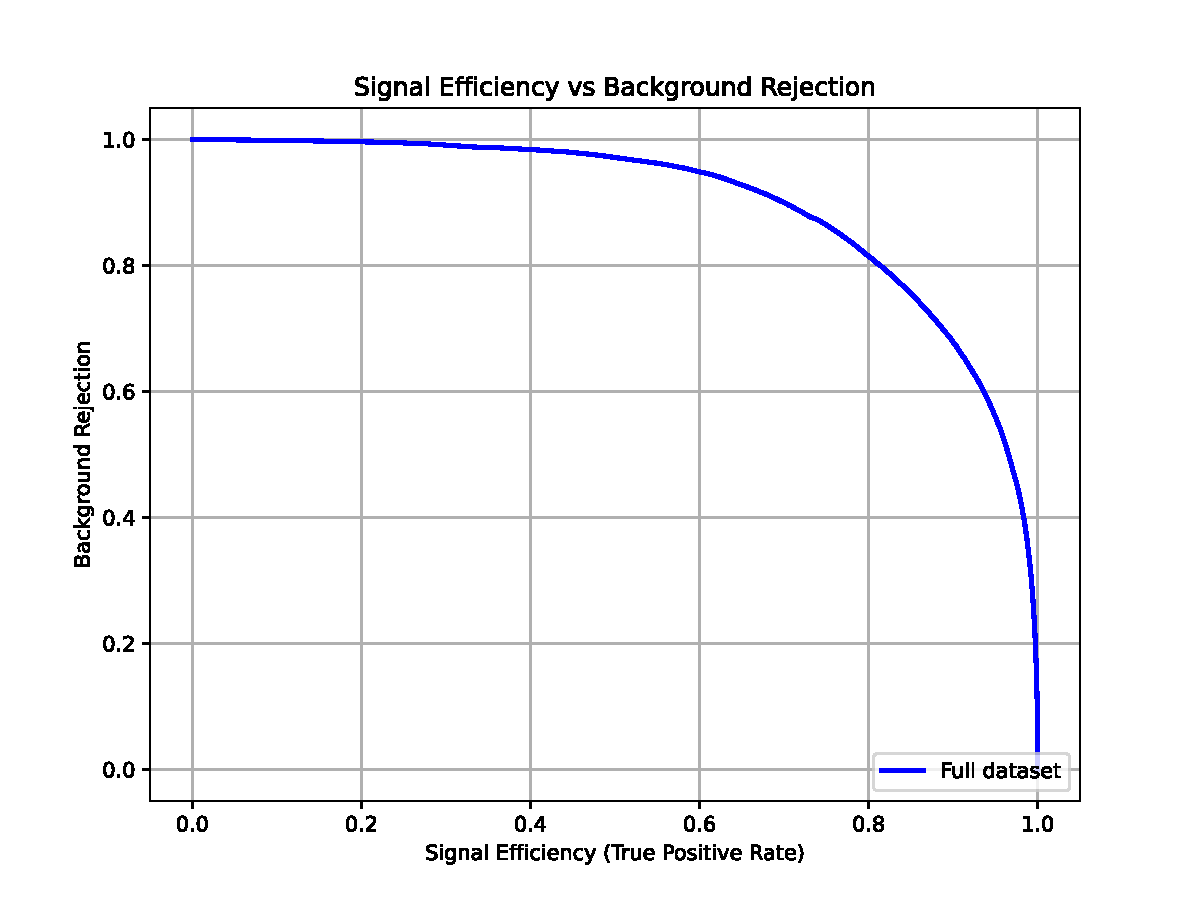
\includegraphics[width=1\linewidth]{res/fig/3-chapter/8-roc-curve.pdf}
            \caption{Curva di ROC dell'allenamento.}
            \label{fig:ROC-curve}
        \end{figure}

\newpage

\begin{comment} 
\section{Futuri sviluppi: applicazione ai dati reali}
\end{comment}